\chapter{Модель картины мира. Семантический уровень} \label{chapt3}

Как было сказано в выводах главы \ref{chapt1}, внутренний, семантический уровень описания картины мира субъекта деятельности с необходимостью должен быть согласован с нейрофизиологическими данными о строении коры головного мозга человека. В данной главе будет введено такое описание с рядом существенных упрощений, призванных облегчить изложение и позволяющих сконцентрироваться на изучении основных свойств возникающих математических объектов. В начале будет дано семантическое определение образной компоненты и процедуры её функционирования в процессе восприятия, а затем будут введены описания остальных компонент знака, синтаксические определения которых давались в главе \ref{chapt2}. В конце главы дано описание одной из основных функций картины мира "--- процедуры образования нового знака на семантическом уровне и приведены результаты исследования итерационного процесса формирования и связывания образа и значения нового знака.

\section{Образная компонента знака}\label{sect3_1}

\subsection{Основные принципы работы образной компоненты} \label{subsect3_1_1}

Рассмотрим объекты, которые возникают при описании моделей зрительного восприятия, построенных на следующих основных принципах:
\begin{enumerate}
	\item иерархичность,
	\item обладание функцией выдвижения перцептивных гипотез,
	\item обладание способностью распознавать как динамические так и статические явления,
	\item управляемость.
\end{enumerate}

Эти принципы согласуются с выводами, сделанными при анализе существующей литературы по нейрофизиологическим данным (см. параграф \ref{sect1_4}). Приведём обоснование выбора именно этих свойств в качестве базовых для построения семантического уровня модели КМ.

Первый принцип был выдвинут в работах когнитивных психологов А. Трисман (A.\,M.~Triesman) и Дж. Джелед (G.~Gelade) \cite{Triesman1980} и заключается в том, что на уровне работы сетчатки имеется набор базовых признаков  или протобъектов (на уровне вторичных зрительных отделов коры головного мозга) \cite{Rensink2000}, из которых в процессе научения образуются более сложные признаки. Из полученных сложных признаков строятся ещё более сложные и т.\,д. При этом процесс восприятия представляет собой последовательную активацию части получающейся иерархии, начиная с базовых признаков и заканчивая сложным объектом, предъявляемым зрительной системе. Основным критерием принадлежности разных признаков одному объекту (сложному признаку) является пространственная и временная когерентность. Иерархичность процесса восприятия, как одного из процессов протекающих в картине мира, также проявляется и в функциональной иерархичности коры головного мозга, что подтверждается большим количеством нейрофизиологических данных \cite{Hawkins2009, Bolotova2011}.

Основной задачей образной компоненты на каждом уровне иерархии, таким образом, становится выявление повторяющихся временных и пространственных шаблонов в поступающем наборе сигналов и низкоуровневых признаков.

По данными анализа движения глаз испытуемых доказано, что любой процесс восприятия, как динамического так и статического явления, представляет собой развёрнутый во времени процесс, каждый этап которого с той или иной степенью точности предсказывается на основе предыдущих этапов \cite{Velichkovsky2006, Hawkins2009}. Именно в этом заключается второй принцип: модель элемента картины мира должна включать в себя процессы выдвижения гипотез о том, какая часть иерархии признаков будет активирована в следующий момент времени.

Третий принцип определяет важность параметра времени: образная компонента должна с самого начала уметь работать с меняющимися во времени признаками, не выделяя явно случай статического изображения. Наконец, четвёртый принцип основан на теории активного зрения и том факте, что каждый этап распознавания признака на каком-либо уровне иерархии в процессе восприятия чередуется с активным этапом моторной реакции. Особенно ярко этот факт проявляется в случае зрительного восприятия при наблюдении саккадических движений глаза.

Учитывая перечисленные принципы, на которых строятся большинство существующих моделей восприятия (не только зрительного), в следующем параграфе вводится определение распознающего автомата, являющегося основным структурным элементом как образной, так и других компонент знака (рис. \ref{fg:sign_rb}). Далее приводится алгоритм работы образной компоненты, исследуется его свойства путём постановки ряда задач распознавания.

\begin{figure}[h]
	\centering
    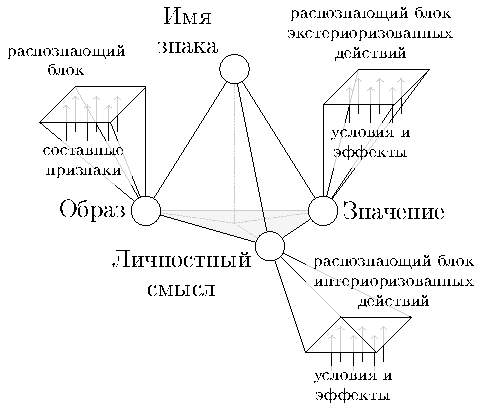
\includegraphics[width=0.7\linewidth]{sign_rb}
    \caption{Знак и его компоненты.}
    \label{fg:sign_rb}
\end{figure}

%============================================================================================================================
\subsection{Распознающий автомат} \label{sect:recogn_block}
Далее рассмотрим автомат $R_i^j$, который будем называть \textit{распознающим автоматом} уровня $j$ с индексом $i$ или просто $R$-автоматом. Опишем кратко его автоматную функцию \cite{Kudryavtcev1985}, а затем определим алгоритм его работы формально.  Для этого воспользуемся понятием \textit{признака}, который будем понимать как составную часть информационного представления некоторой сущности, явления или процесса \cite{Vapnik1974}.

Каждый распознающий автомат распознает или, применительно к~низкоуровневым сигналам, измеряет, некоторые признаки на основе входного вектора данных.  Процесс распознавания (измерения) заключается в сопоставлении признака взвешенному значению, который определяет уровень доверия тому, насколько успешно удалось построить (измерить) признак из составляющих его низкоуровневых признаков, информация о которых содержится во входном векторе. Такой вес будем называть \textit{весом признака} во входном векторе.

Входной вектор, в свою очередь, представляет собой взвешенный вектор низкоуровневых признаков, по которым распознаются выходные признаки. Распознающий автомат обладает множеством состояний, каждое из которых представляет собой также взвешенный вектор входных признаков, но в следующий момент времени. Такой вектор будем называть \textit{вектором ожиданий}. Опишем сказанное более строго.

Пусть заданы множества $\mathcal R$ и $\mathcal F$. Множество $\mathcal R$ будем называть совокупностью распознающих автоматов, а множество $\mathcal F$ "--- совокупностью допустимых признаков. Введём бинарное отношение $\dashv$, определённое на паре множеств $\mathcal F$ и $\mathcal R$, и будем читать $f_k{\dashv}R_i^j$, $f_k\in\mathcal F$, как <<признак $f_k$ распознаётся $R$-автоматом $R_i^j$>> или как <<признак $f_k$ измеряется $R$-автоматом $R_i^j$>>. Множество всех распознаваемых $R$-автоматом $R_i^j$ признаков будем обозначать $F_i^{*j}$, т.е. ${\forall}f^*{\in}F_i^{*j} f^*{\dashv}R_i^j, F_i^{*j}{\subseteq}\mathcal F$.

Рассмотрим связный ориентированный (ярусный) граф $G_R=(V,E)$, где $V=\mathcal R$ "--- множество вершин, $E\subset \mathcal R\times \mathcal R$ "--- множество рёбер. Каждая вершина $v$, принадлежащую $j$-ому ярусу графа $G_R$, является распознающим автоматом $R_{i_1}^{j_1}$ уровня $j_1$, а ребро $e=(R_{i_1}^{j_1},R_{i_2}^{j_2}){\in}E$ обозначает  иерархическую связь между $R$-автоматом $R_{i_1}^{j_1}$ и $R$-автоматом $R_{i_2}^{j_2}$. $R$-автомат $R_{i_1}^{j_1 }$ в данном случае будем называть дочерним, а $R$-автомат $R_{i_2}^{j_2}$ "--- родительским (рис. \ref{fg:rb_hier}).

\begin{figure}[h]
	\centering
	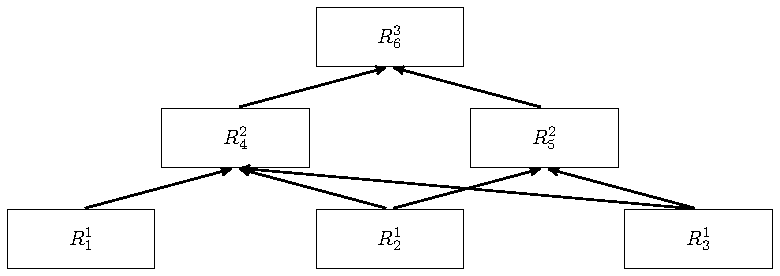
\includegraphics[width=0.7\linewidth]{rb_hierarchy}
	\caption{Пример иерархии распознающих автоматов. Так, узел $R_{i_2}^{j_2}$ является родительским распознающим автоматом, а узел $R_{i_1}^{j_1}$ "--- дочерним автоматом.}
	\label{fg:rb_hier}
\end{figure}

Рассмотрим распознающий автомат $R_i^j$. Определим множество $F_i^j{\subseteq}\mathcal F$ таких признаков, что для любого $f{\in}F_i^j$ существует распознающий автомат $R_k^{j-1}$ уровня $j-1$, дочерний по отношению к $R$-автомату $R_i^j$, такой, что $f{\dashv}R_k^{j-1}$. Такое множество $F_i^j$ будем называть совокупностью входных признаков распознающего автомата $R_i^j$. Для каждого признака $f^*{\in}F_i^{*j}$ введём функцию распознавания $\hat{f}(x_1,\dots,x_q )=x^*$, где $x^*{\in}[0,1]$ "--- вес распознаваемого признака $f^*$ в выходном векторе, а $x_1,\dots,x_q{\in}[0,1]$ "--- веса признаков из множества $F_i^j$ в текущем входном векторе. Множество таких функций для распознающего автомата $R_i^j$ обозначим как $\hat{F}_i^j$.

Пусть мощность множества распознаваемых признаков $F_i^{*j}$ и множества функций распознавания $\hat{F}_i^j$ равна $l_i^j$, а мощность множества входных признаков $F_i^j$ равна $q_i^j$. Введём упорядоченное множество локальных моментов времени $T_i^j$ для распознающего автомата $R_i^j$. Будем называть \textit{вычислительным циклом} полуинтервал между соседними моментами времени поступления сигналов обратной связи с верхнего уровня иерархии (см. ниже). Для каждого распознающего автомата определим характерное время $h_i^j$, за которое выполняется один цикл вычисления. 

В начале $s$-ого цикла вычисления (момент времени $\tau_s\in{T_i^j}$)  распознающий автомат $R_i^j$ получает на вход вектор длины $l_i^j$ ожиданий $\hat{x}_i^{j+1}(\tau_s)$, вычисляемый по формуле среднего от векторов ожиданий, поступающих от родительских относительно $R$-автомата $R_i^j$ распознающих автоматов $R_k^{j+1}$:
\begin{equation}
	\hat{x}_i^{j+1}(\tau_s)=\frac{1}{N_i^j}\sum_{k{\in}K_i^{j+1}}\hat{x}_k^{j+1}(\tau_s),
\end{equation}
где $N_i^j$ - количество родительских $R$-автоматов, $K_i^{j+1}$ - множество индексов родительских относительно $R_i^j$ распознающих автоматов. Далее в~каждый момент времени $t\in{T_i^j}$, $\tau_s\leqslant{t}\leqslant\tau_s+h_i^j$,  распознающий автомат $R_i^j$ получает на~вход взвешенный вектор $\bar{x}_i^j(t)$ входных признаков из~множества $F_i^j$ длины $l_i^j$, вычисляет выходной взвешенный вектор $\bar{x}_i^{*j}(t)$ распознаваемых признаков из~множества $F_i^{*j}$ длины $l_i^j$, вычисляет вектор ожиданий $\hat{x}_i^j(t)$ входных признаков в следующий момент времени длины $q_i^j$ (рис.~\ref{fig:rb_cycle}). Параметр $h_i^j$ , таким образом, служит характеристикой глубины памяти $R$-автомата.
	
\begin{figure}[h]
	\centering
	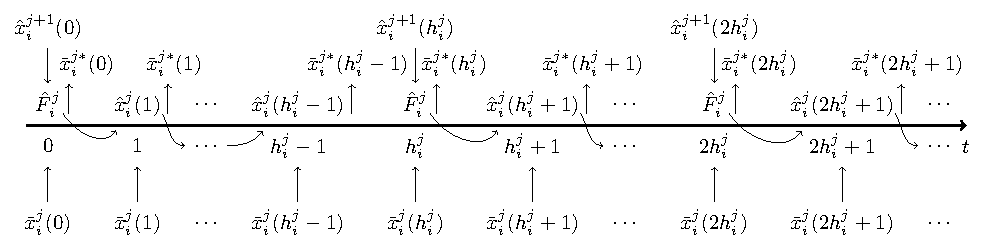
\includegraphics[width=1.0\linewidth]{rb_cycle}
	\caption{Вычислительные циклы распознающего автомата. В моменты времени $0,h_i^j,2h_i^j,\dots$ происходит определение нового начального состояния.}
	\label{fig:rb_cycle}  
\end{figure}

\subsection{Алгоритм $\mathfrak A_{th}$ работы распознающего автомата}\label{subsect:rb_algorithm}

Будем рассматривать распознающий автомат $R_i^j$ как автомат с конечным множеством состояний. Для этого каждой функции распознавания $\hat{f}_k$ из множества $\hat{F}_i^j$ будем ставить в соответствие набор \textit{матриц предсказания} $Z_k=\{Z_1^k,…,Z_m^k\}$ размерности $q_i^j\times h_i^j$, где $h_i^j$ "--- характерное время распознающего автомата $R_i^j$. Столбец $\bar{z}_u^r=(z_{u1}^k,…,z_{uq}^k)$ матрицы $Z_r^k$ интерпретируется как вектор предсказания присутствия входных признаков из множества $F_i^j$ в момент времени $\tau_s+u$, при этом $z_{uv}^k\in\{0,1\}$, т.е. вектор $\bar{z}_u^r$ является булевым вектором. Сама матрица $Z_r^k$ задаёт, таким образом, последовательность событий, наличие которых свидетельствует о~присутствии распознаваемого функцией $\hat{f}_k$ признака. Множество всех матриц предсказания распознающего автомата $R_i^j$ будем обозначать как $\mathcal{Z}_i^j$.

Таким образом, $R$-автомат $R_i^j$ является бесконечным автоматом Миля с переменной структурой и конечной памятью и определяется следующим набором $R_i^j=<X_i^j\times \hat{X}_i^{j+1}, 2^{\mathcal Z_i^j}, X_i^{*j}\times \hat{X}_i^j,\varphi_i^j,\vec\eta_i^j,>$, где
\begin{itemize}
	\item $X_i^j$ "--- множество входных сигналов (пространство векторов длины $q_i^j$ действительных чисел от $0$ до $1$), 
	\item $X_i^{*j}$ "--- множество выходных сигналов (пространство векторов длины $l_i^j$ действительных чисел от $0$ до $1$), 
	\item $\hat{X}_i^{j+1}$ "--- множество управляющих сигналов с верхнего уровня иерархии (пространство векторов длины $l_i^j$ действительных чисел от $0$ до $1$),
	\item $\hat{X}_i^j$ "--- множество управляющих сигналов на нижний уровень иерархии (пространство векторов длины $q_i^j$ действительных чисел от $0$ до $1$),
	\item $2^{\mathcal Z_i^j}$ "--- множество состояний (множество подмножеств множества матриц предсказания),
	\item $\varphi_i^j:X_i^j\times \hat{X}_i^{j+1}\to 2^{\mathcal Z_i^j}$ "--- функция переходов,
	\item $\vec\eta_i^j:2^{\mathcal Z_i^j} \to X_i^{*j}\times \hat{X}_i^j$ "--- вектор"--~функция выходов.
\end{itemize}

Для удобства определения автоматной функции обозначим \textit{входное воздействие} через $\omega_i^j:T{\to}X_i^j$, а \textit{выходную величину} через $\gamma_i^j:T{\to}X_i^{*j}$ как это принято в~теории динамических систем \cite{Kalman1971, KalmanE1971} (рис.~\ref{fig:rb_io}).

\begin{figure}[h]
	\centering
	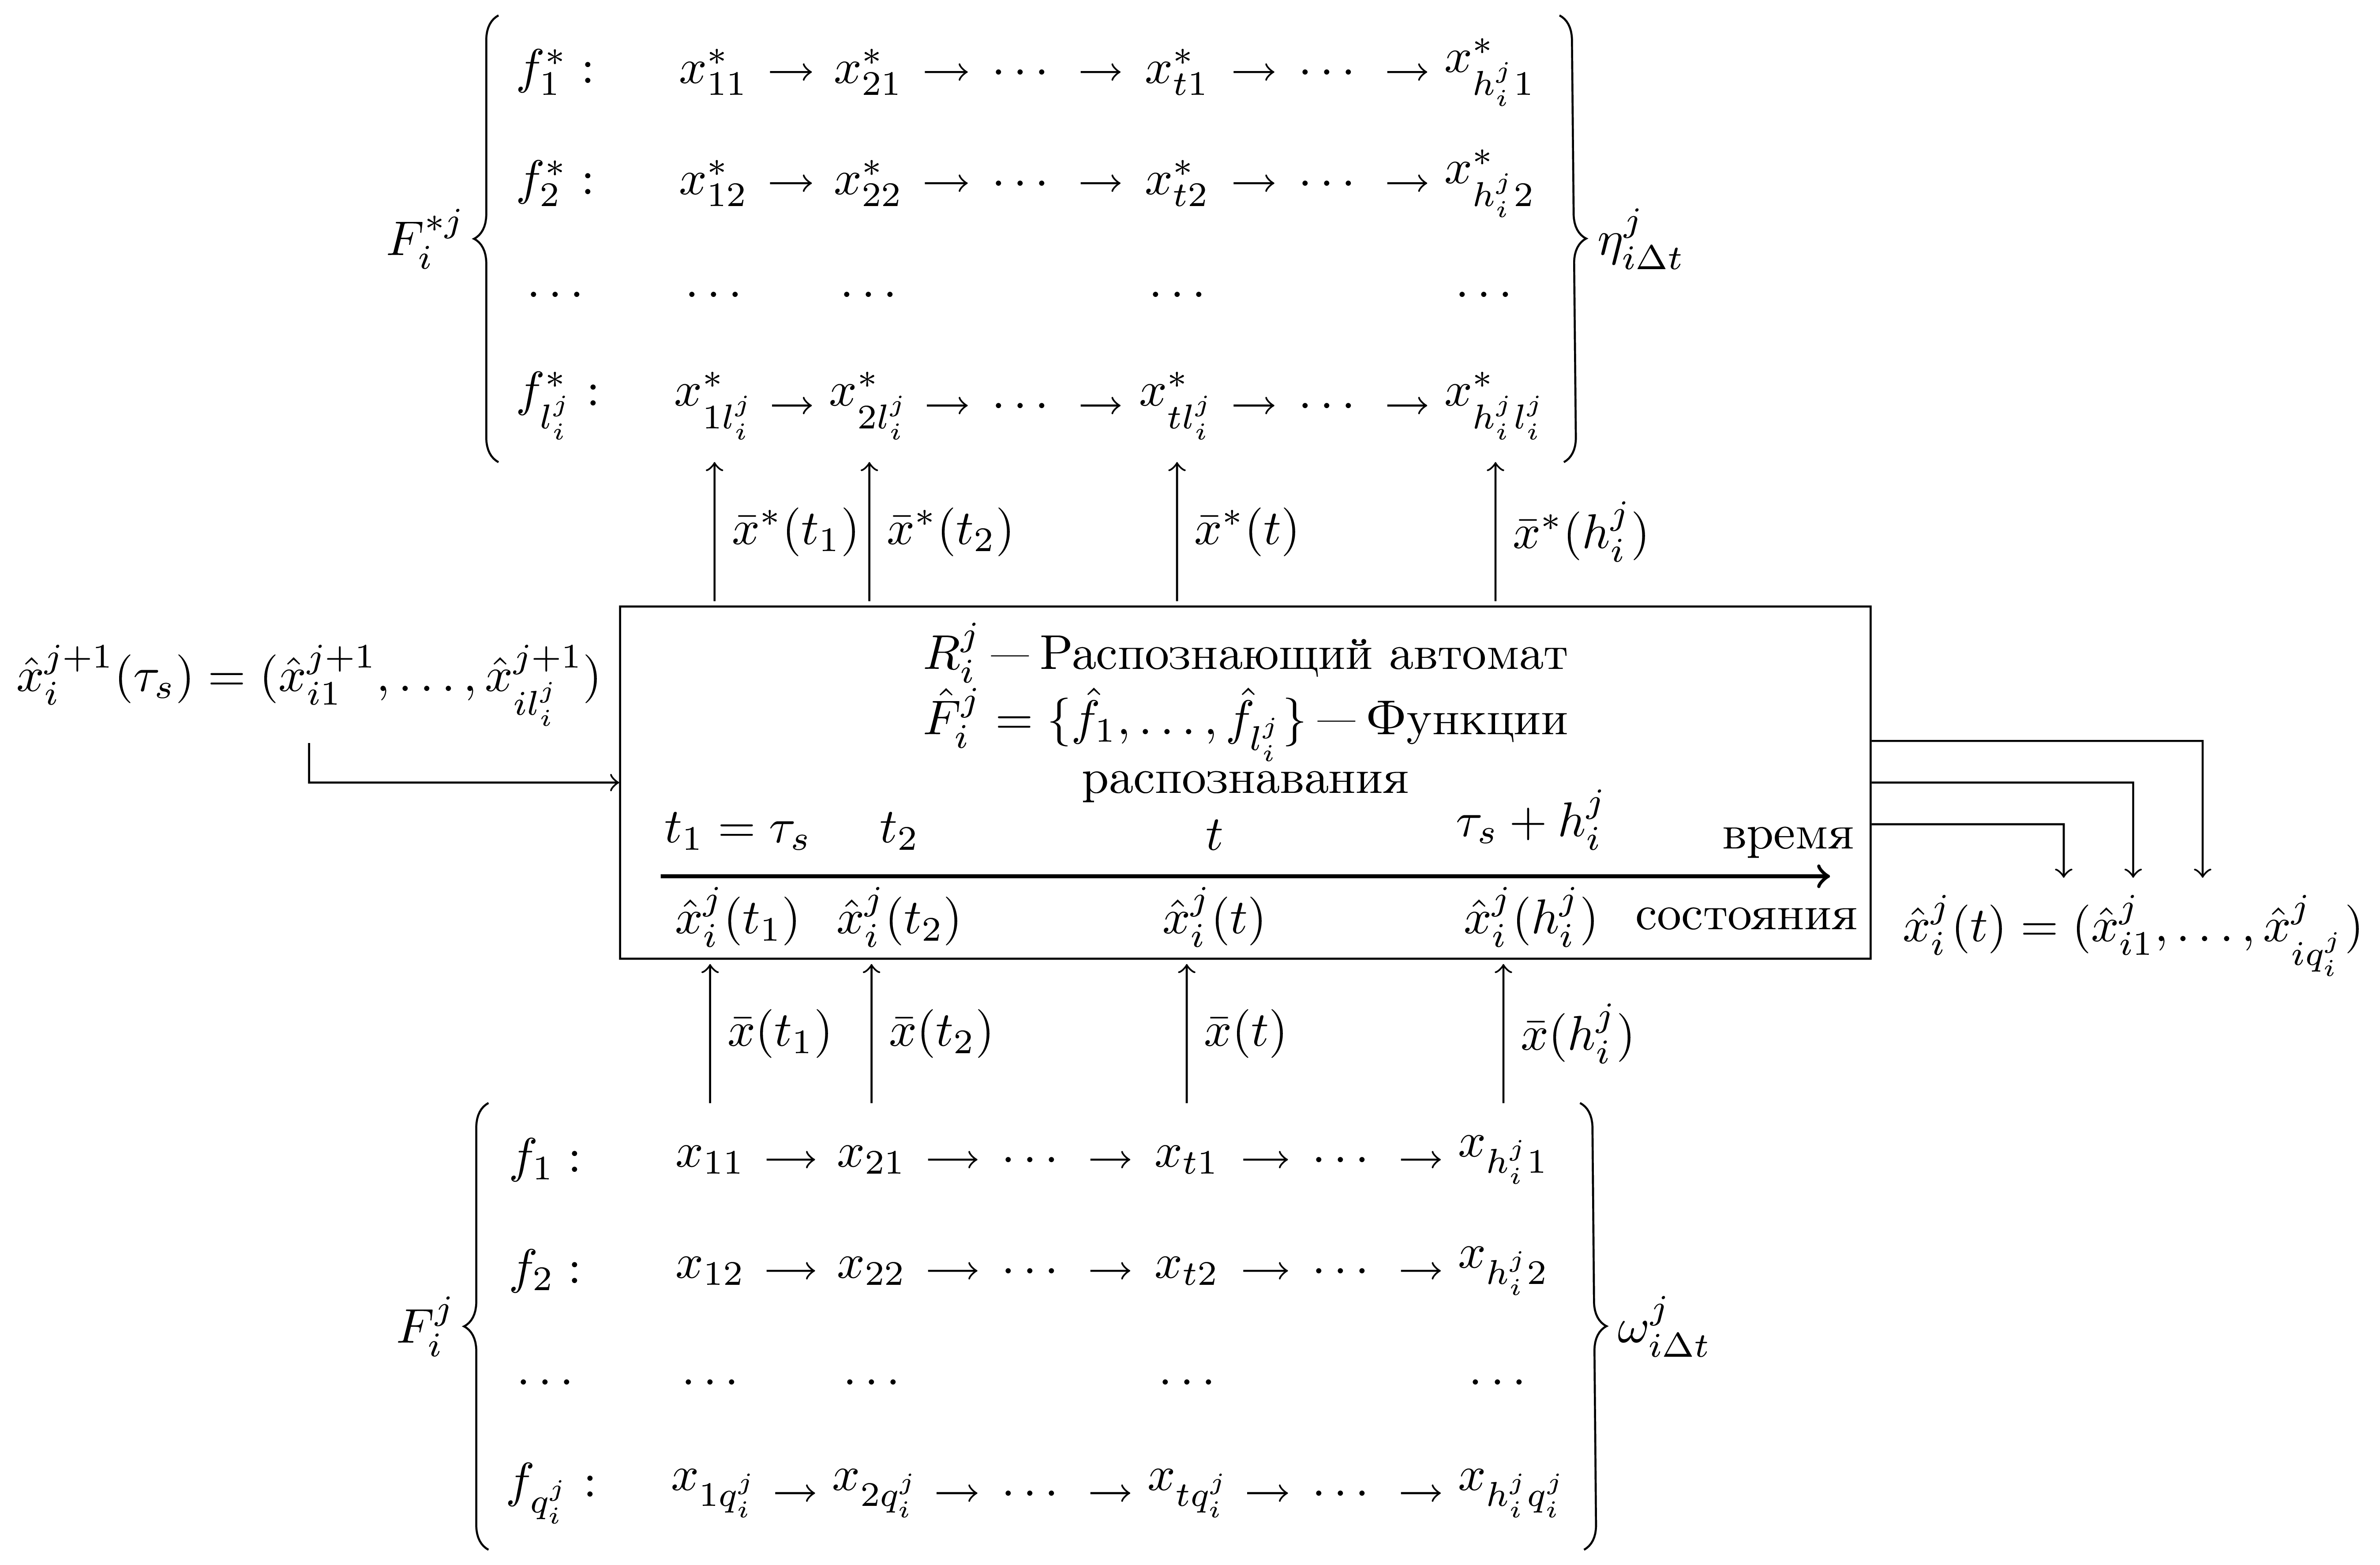
\includegraphics[width=\linewidth]{rb_io}
	\caption{Схема входных и выходных отображений распознающего автомата.}
	\label{fig:rb_io}
\end{figure}

На страницах \pageref{alg:th_init} и \pageref{alg:th_cycle} приведён алгоритм $\mathfrak{A}_{th}$ вычислительного цикла распознающего $R$-автомата, в котором рассчитываются значения функции переходов $\varphi_i^j(\hat{x}_i^{j+1}(\tau_s+t),\omega_i^j)$, $1\leqslant{t}\leqslant h_i^j-1$, и выходной функции $\vec\eta_i^j(\mathcal Z_i^{*j}(\tau_s+t))$, $1\leqslant{t}\leqslant h_i^j-1$, $\mathcal Z_i^{*j}(\tau_s+t)$ "--- текущее состояние. В алгоритме используется функция $W$ нормировки весовых значений:
\begin{equation}
	W(\bar x)=\left(\frac{x_1}{\max\limits_i x_i},\dots,\frac{x_n}{\max\limits_i x_i}\right),
\end{equation} 
где $\bar x=(x_1,\dots,x_n)$ "--- вектор с ненормированными компонентами. Кратко опишем шаги алгоритма.

Вычислительный цикл распознающего автомата начинается с определения начального состояния при~помощи управляющего воздействия с верхних уровней иерархии "--- вектора ожиданий $\hat x_i^{j+1}(\tau_s)$ (шаги \ref{alst:init_start}--\ref{alst:init_end}). Начальное состояние определяется как подмножество таких распознаваемых признаков множества $F_i^{*j}$, которые предсказываются на основе состояния $R$-автоматов верхнего уровня. Первая константа $c_1$ определяет порог предсказываемого веса распознаваемых признаков, вышей которого соответствующие функции распознавания попадают во множество активных функций $\hat F^*$ (шаг \ref{alst:select_f}). Далее производится отбор тех матриц предсказания активных функций распознавания, для которых обычное расстояние по норме $\|x\|=\sum_i |x_i|$ первого столбца $\bar z_1^r$ от входного вектора $\bar z_i^j$ в начальный момент времени не превышает второй константы $c_2$ (шаг \ref{alst:select_z}). Множество полученных таким образом активных матриц предсказания и является текущим состоянием распознающего автомата (шаг \ref{alst:init_state}). На основе активных матриц предсказания методом голосования вычисляется выходной вектор в начальный момент времени $\bar x_i^{j*}(\tau_s)$ (шаги \ref{alst:init_calc_out2} -- \ref{alst:init_calc_out3}).

\begin{algorithm}[H]
	\caption{Алгоритм $\mathfrak{A}_{th}$ (часть I, задание начального состояния)}\label{alg:th_init}
	\begin{algorithmic}[1]
				\Require $\tau_s, \hat{x}_i^{j+1}(\tau_s), \omega_i^j$.
		\Ensure $\varphi_{i\Delta t}^j, \vec\eta_{i\Delta t}^j$.

		\State $\hat{F}^*=\varnothing,Z^*=\varnothing,t=0$; \Comment{активные функции распознавнаия и матрицы предсказания}
		\State $c_1\in(0,1), c_2\in(0,1)$; \Comment{пороговые константы}

		\Statex \Comment{определение начального состояния}
				
		\ForAll{компонент $\hat{x}_{ik}^{j+1}$ вектора $\hat{x}_i^{j+1}(\tau_s)=(\hat{x}_{i1}^{j+1},\hat{x}_{i2}^{j+1},\dots,\hat{x}_{il}^{j+1})$} \label{alst:init_start}
			\If{$\hat{x}_{ik}^{j+1}{\ge}c_1$} \label{alst:select_f}
				\State $\hat{F}^*:=\hat{F}^*\cup\{\hat{f}_k\}$;
			\EndIf
		\EndFor
		
		\State $\bar x_i^j:=\omega_i^j(\tau_s)$;
		
		\ForAll{функций распознавания $\hat{f}_k\in\hat{F}^*$}
			\ForAll{$Z_r^k\in Z_k$, соответствующих функции распознавания $\hat{f}_k$,}
				\If{$\frac{\|\bar{z}_1^r-\bar{x}_i^j\|}{\|\bar{z}_1^r\|+\|\bar{x}_i^j\|}<c_2$} \label{alst:select_z}
					\State $Z^*:=Z^*\cup\{Z_r^k\}$;
				\EndIf
			\EndFor
		\EndFor
		
		\State $\varphi_i^j(\bar x_i^j,\hat{x}_i^{j+1}(\tau_s)) := Z^*$; \Comment{значение функции переходов в начальный момент времени}\label{alst:init_state}
		\State $\bar N:=(|\{Z_r^1|Z_r^1\in Z^*\}|,\dots,|\{Z_r^{l_i^j}|Z_r^{l_i^j}\in Z^*\}|)$; \label{alst:init_calc_out2}
		\State $\eta(Z^*)=\bar{x}_i^{*j}:=W(\bar N)$; \Comment{значение функции выходов в начальный момент времени} \label{alst:init_calc_out3}
		\State $\hat x_i^j=W(\sum_{\hat f_k\in\hat F^*}\hat x_{ik}^{j+1}\sum_{Z_r^k\in Z^*}\bar z_2^r)$;\label{alst:init_control}
		\label{alst:init_end}
		\algstore{algst:store1}
	\end{algorithmic}
\end{algorithm}
	
Вектор управления $\hat x_i^j(\tau_s+1)$ определяется как нормированный вектор, $s$-ый компонент которого равен сумме всех $s$-ых элементов вторых колонок активных матриц предсказания с весами, соответствующими элементам вектора ожиданий $\hat x_i^{j+1}(\tau_s)$ (шаг \ref{alst:init_control}). Т.~к. используется представление о будущем входном сигнале (вторая колонка матриц предсказания), то $\hat x_i^j(\tau_s+1)$ играет роль предсказывающего вектора для нижних уровней иерархии.

После определения начального состояния начинает выполняться тело основного цикла, в котором до тех пор, пока время не превысит характерное время распознающего автомата $h_i^j$ повторяется вычисление выходного вектора и состояния в следующий момент времени (шаги \ref{alst:cycle_start}--\ref{alst:cycle_end}). В начале обновляется состояние, т.~е. множество активных матриц предсказания $Z^*$, за счёт удаления тех матриц, соответствующие столбцы которых достаточно сильно отличаются от текущего входного вектора $\bar x_i^j$ (шаг \ref{alst:update_z}). Далее методом голосования по количеству матриц в множестве активных матриц предсказания, отвечающих за соответствующий выходной признак, вычисляется выходной вектор $\bar x_i^{j*}$ (шаги \ref{alst:calc_out1}--\ref{alst:calc_out3}).

\begin{algorithm}[H]
	\caption{Алгоритм $\mathfrak{A}_{th}$ (часть II, основной цикл)}\label{alg:th_cycle}
	\begin{algorithmic}[1]
		\algrestore{algst:store1}
			\Statex \Comment{основной цикл}
	
	\State $t=1$;
	\While{$t\leqslant{h_i^j}-1$} \label{alst:cycle_start}
		\State $\bar{x}_i^j:=\omega(\tau_s+t)$;
	
		\ForAll{матриц предсказания $Z_r^k$ из множества $Z^*$}
			\If{$\frac{\|\bar{z}_{t+1}^r-\bar{x}_i^j\|}{\|\bar{z}_{t+1}^r\|+\|\bar{x}_i^j\|}\geqslant{c_2}$} \label{alst:update_z}
				\State $Z^*:=Z^*\setminus\{Z_r^k\}$;
			\EndIf
		\EndFor
	
		\State $\varphi_i^j(\bar x_i^j,\hat{x}_i^{j+1}(\tau_s)) := Z^*$; \Comment{значение функции переходов в момент времени $t$}
		\State $\bar N=(|\{Z_r^1|Z_r^1\in Z^*\}|,\dots,|\{Z_r^{l_i^j}|Z_r^{l_i^j}\in Z^*\}|)$; \label{alst:calc_out1}
		\State $\eta(Z^*)=\bar{x}_i^{*j}:=W(\bar N)$;\Comment{значение функции выходов в момент времени $t$} \label{alst:calc_out3}
	
		\State $t=t+1$;
		\If{$t\leqslant{h}_i^j-2$}
			\State $\hat{x}_i^j:=W(\sum_{\hat f_k\in\hat F^*}\hat x_{ik}^{j+1}\sum_{Z_r^k\in Z^*}\bar z_t^r)$; \label{alst:calc_state1}
		\EndIf
	\EndWhile \label{alst:cycle_end}
	\end{algorithmic}
\end{algorithm}
		
В завершение тела основного цикла вычисляется выходной управляющий вектор ожиданий в следующий момент времени $\hat x_i^j(\tau_s+t+1)$. Как и на этапе определения начального состояния, вектор ожиданий равен нормированному вектору, элементы которого равны сумме элементов столбцов всех активных матриц предсказания, соответствующих текущему моменту времени с учётом весов начального управляющего вектора $\hat x_i^{j+1}(\tau_s)$ (шаг \ref{alst:calc_state1}).

\section{Исследование алгоритма $\mathfrak A_{th}$ работы образной компоненты}\label{sect3_2}

Для обоснования корректности сформулированного алгоритма работы образной компоненты знака, в данном параграфе будет поставлен рад задач распознавания (классификации) и построены множества операторов распознавания. Корректность алгоритма будет продемонстрирована за счёт корректности данных множеств операторов распознавания.

\subsection{Статическая задача классификации}

\subsubsection{Начальный момент времени}
В начале рассмотрим статический случай, т.~е. зафиксируем момент времени $t$, равный началу некоторого $s$-го вычислительного цикла $\tau_s$. В этом случае, распознающий автомат $R_i^j$ можно рассматривать как \textit{статический оператор распознавания} $R_i^j(\hat{x}_i^{j+1},\mathcal{Z}_i^j,\bar{x}_i^j)=\bar{x}_i^{*j}$. Напомним, что $\bar{x}_i^{*j}$ "--- это взвешенный вектор распознаваемых признаков $f_1^*,\dots,f_l^*$ из множества $F_i^{*j}$. Далее кратко будем записывать $R^0(\hat{x},\mathcal{Z},\bar{x})=\bar{x}^*$ и везде, где это возможно, будем опускать индексы $j$ и $i$.
	
Введём совокупность задач $\mathcal Q^0$ аналогично работе \cite{Zhuravlev1977,ZhuravlevE1977}. Задача $Q^0(\hat{x},\bar{x},\alpha_1,\dots,\alpha_l)\in\mathcal Q^0$ состоит в построении оператора, вычисляющего по поступившему вектору ожиданий $\hat{x}$ и входному вектору $\bar{x}$ значения $\alpha_1,\dots,\alpha_l\in\{0,1\}$ присутствия признаков $f_1^*,\dots,f_l^*$. Другими словами, искомый алгоритм $A^{0*}$ переводит набор $(\hat{x},\bar{x})$ в вектор $\bar{\alpha}=(\alpha_1,\dots,\alpha_l)$, который будем называть \textit{информационным вектором} входного вектора $\bar{x}$ (рис. \ref{fig:rb_correct_stat0}).
	
\begin{figure}[h]
	\centering
	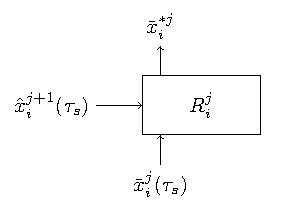
\includegraphics[width=0.5\linewidth,page=1]{rb_correct}
	\caption{Статическая схема корректности для момента времени $\tau_s$.}
	\label{fig:rb_correct_stat0}
\end{figure}

Пусть множество $\mathcal A^0$ состоит из алгоритмов, переводящих пары $(\hat{x},\bar{x})$ в векторы $\bar{\beta}$, составленные из элементов $0,1,\Delta:A(\hat{x},\bar{x})=\bar{\beta}$. Если $\beta_i\in\{0,1\}$, то $\beta_i$ "--- значение величины $\alpha_i$, вычисленное алгоритмом $A$. Если $\beta_i=\Delta$, то алгоритм $A$ не вычислил значение $\alpha_i$ информационного вектора $\bar\alpha$.
	
\begin{Def}
	Алгоритм $A^0$ называется корректным для задачи $Q^0$, если выполнено равенство
	\begin{equation}
		A^0(\hat{x},\bar{x})=\bar{\alpha}.
	\end{equation}
	Алгоритм $A$, не являющийся корректным для $Q^0$, называется некорректным.
\end{Def}

Далее будем считать, что множество $\mathcal A^0$ является совокупностью, вообще говоря, некорректных алгоритмов.
	
\begin{Pred}[аналог теоремы Журавлёва о введении пространства оценок из \cite{Zhuravlev1977}]
	\label{pred:decompositon}
	Каждый алгоритм $A^0\in\mathcal A^0$ представим как последовательность выполнения алгоритмов $R^0$ и $C^0$, где $R^0(\hat{x},\bar{x})=\bar{x}^*$, $\bar{x}^*$ "--- вектор действительных чисел, $C^0(\bar{x}^*)=\bar{\beta}$, $\beta_i\in\{0,1,\Delta\}$.
\end{Pred}
	
\begin{Proof}
	Пусть $D$ "--- алгоритм перехода вектора $\bar{\beta}$ к числовому вектору $\bar{y}$. В качестве $D$ можно рассмотреть, например, $y_i=\beta_i$, если $\beta_i\in\{0,1\}$, и $y_i=1/2$, если $\beta_i=\Delta$. Очевидно, что существует обратный алгоритм $D^{-1}$ перехода от $\bar{y}$ к $\bar{\beta}$. Положим $R^0=A^0\cdot D$, $C^0=D^{-1}$. Тогда очевидно, что $A^0=R^0\cdot C^0=(A^0\cdot D)\cdot D^{-1}=A^0$.
\end{Proof}

Из утверждения \ref{pred:decompositon} следует, что множество алгоритмов $\mathcal A^0$ порождает множества $\mathcal R^0$ и $\mathcal C^0$, которые будем называть \textit{множеством операторов распознавания} и \textit{множеством решающих правил}, соответственно. В качестве операторов из множества $\mathcal R^0$ будем рассматривать операторы $R^0(\hat x,\mathcal Z,\bar x)$.
	
\begin{Def}
	Решающее правило $C^{0*}$ называется корректным на множестве входных векторов $X$, если для всякого вектора $\bar x$ из $X$ существует хотя бы один числовой вектор $\bar x^*$ такой, что $C^{0*}(\bar x^*)=\bar\alpha$, где $\bar\alpha$ "--- информационный вектор входного вектора $\bar x$.
\end{Def}

В множестве операторов $\mathcal R^0$ введём операции умножения на скаляр, сложения и умножения. Пусть $r'$ "--- скаляр, $R',R''\in\mathcal R^0$. Определим операторы $r'\cdot R'$, $R'+R''$ и $R\cdot R''$ следующим образом:
	
\begin{equation}
\label{eq:oper_scalar}
	r'{\cdot}R'=(r'{\cdot}{x_1^*}',\dots,r'{\cdot}{x_l^*}'),
\end{equation}

\begin{equation}
\label{eq:oper_sum}
	R'+R''=({x_1^*}'+{x_1^*}'',\dots,{x_1^*}'+{x_l^*}''),
\end{equation}

\begin{equation}
\label{eq:oper_mult}
	R'{\cdot}R''=({x_1^*}'{\cdot}{x_1^*}'',\dots,{x_1^*}'{\cdot}{x_l^*}'').
\end{equation}
	
\begin{Pred}
	Замыкание $L(\mathcal R^0)$ множества $\mathcal R^0$ относительно операций \eqref{eq:oper_scalar} и \eqref{eq:oper_sum} является векторным пространством.
\end{Pred}

\begin{Def}
	Множество $L(\mathcal A^0)$ алгоритмов $A^0=R^0\cdot C^{0*}$ таких, что $R^0\in L(\mathcal R^0)$, называются линейным замыканием множества $\mathcal A^0$.
\end{Def}

Зафиксируем пару $(\hat{x},\bar{x})$ вектора ожидания и входного вектора. Аналогично \cite{Zhuravlev1977} будем рассматривать задачи $Q^0(\hat{x},\bar{x})$, обладающие следующим свойством относительно множества операторов распознавания $\mathcal R^0$.
	
\begin{Def}
	Если множество векторов $\{R^0(\hat{x},\bar{x})|R^0\in\mathcal R^0\}$ содержит базис в пространстве числовых векторов длины $l$, то задача $Q^0(\hat x,\bar x,\bar\alpha)$ называется полной относительно $\mathcal R^0$.
\end{Def}

\begin{Pred}[аналог теоремы Журавлёва о корректности линейного замыкания из \cite{Zhuravlev1977}]
	\label{pred:correctness}
	Если множество задач $\mathcal Q^0$ состоит лишь из задач, полных относительно $\mathcal R^0$, то линейное замыкание $L(\{R^0\cdot C^{0*}|R^0\in\mathcal R^0\})$ ($C^{0*}$ "--- произвольное фиксированное корректное решающее правило) является корректным относительно $\mathcal Q$.
\end{Pred}

\begin{Corollary}
	Пусть $\mathcal A^0$ "--- совокупность некорректных алгоритмов, $\mathcal R^0$ "--- соответствующее множество операторов распознавания, $C^{0*}$ "--- фиксированное корректное решающее правило. Тогда $L(\mathcal A^0)=L(\{R^0\cdot C^{0*}|R^0\in\mathcal R^0\})$ является корректным относительно множества задач $\mathcal Q^0$, если $\mathcal Q^0$ состоит из задач, полных относительно $\mathcal R^0$.
\end{Corollary}

Будем рассматривать только такие задачи $Q^0(\hat{x},\bar{x},\bar{\alpha})$, для которых удовлетворяется следующее условие: ${\exists}k$ такое, что $x_k$ является $k$-ым элементом вектора $\bar{x}$ и $x_k>1/2$. Такое условие является естественным, иначе вектор $\bar{x}$, в котором отсутствуют веса большие $1/2$, не может рассматриваться как достоверный с точки зрения порогового алгоритма $\mathfrak A_{th}$.
	
\begin{Theorem}
	\label{th:correctness}
	Линейное замыкание $L(\mathcal A^0)$ семейства алгоритмов $\mathcal A^0=\{R^0\cdot C^{0*}|R^0\in\mathcal R\}$ с произвольным корректным решающим правилом $C^*$ и операторами распознавания $\mathcal R$, определёнными шагами \ref{alst:init_start}--\ref{alst:init_end} алгоритма $\mathfrak A_{th}$, является корректным на множестве задач $\mathcal Q^0$.
\end{Theorem}

\begin{Proof}
	В силу утверждения \ref{pred:correctness} достаточно доказать, что произвольная задача $Q^0\in\mathcal Q^0$ является полной относительно $\mathcal R^0$. Доказательство полноты $Q^0$ состоит в прямом построении операторов $R_k, k=1,2,\dots,l$ из $L(\mathcal R^0)$, переводящих пару $(\hat{x},\bar{x}), \hat{x}=(\hat{x}_1,\dots,\hat{x}_l), \bar{x}=(x_1,\dots,x_q)$ в числовой вектор
	\begin{equation} \label{crit:fillness}
		\bar{x}_k^*=(x_{k1}^*,\dots,x_{kl}^*),\ x_{kk}^*=1,\ \forall u\neq k\ x_{ku}^*=0.
	\end{equation} 
	
	Пусть мощность множества $\mathcal Z_k$ признака $f_k$ равна $N$, норма $\|\bar x\|$ равна $M{\leqslant}q$, максимальная компонента вектора $\bar{x}$ равна $x_{max}$. Зафиксируем величину $k$ и коэффициенты $c_1=\min_v\hat x_v, c_2=\frac{M}{1+M}$. Рассмотрим матрицы предсказания из множеств $\mathcal{Z}_1,\dots,\mathcal{Z}_l$ признаков $f_1,\dots,f_l$, удовлетворяющие следующим условиям:
	
 \begin{enumerate}
	 	\item в каждой матрице предсказаний $Z_r^k\in\mathcal Z_k$ в столбце $\bar{z}_1^r=(z_{11}^r,\dots,z_{1q}^r)$ компонента $z_{1v}^r=1$, если $x_v=x_{max}$, и $z_{1v}^r=0$, если $x_v<x_{max}$; \label{cond:ii}
	 	
	 	\item в каждой матрице предсказаний $Z_r^u\in\mathcal Z_u, u\neq k$ в столбце $\bar{z}_1^r=(z_{11}^r,\dots,z_{1q}^r)$ компонента $z_{1v}^r=0$ при любых $v$. \label{cond:ij}
 \end{enumerate}
 
 Вычислим величину $x_{kk}^*$. Т.~к. $c_1=\min_u\hat x_u$, то условие $\hat x_k\geqslant c_1$ на шаге \ref{alst:select_f} алгоритма $\mathfrak A_{th}$ автоматически выполняется и функция измерения $\hat f_k$ попадает в множество $\hat F^*$. Из условия \ref{cond:ii} следует, что каждая матрица $Z_r^k\in\mathcal Z_k$ попадает в множество $Z^*$ на шаге \ref{alst:select_z} алгоритма $\mathfrak A_{th}$:
 \begin{equation}
 	\frac{\|\bar{z}_1^r-\bar{x}\|}{\|\bar{z}_1^r\|+\|\bar{x}\|}<\frac{\sum_v|z_{1v}^r-x_v|}{1+M}<\frac{M}{1+M}=c_2,
 \end{equation}
 так как минимум один компонент в $\bar{z}_1^r$ равен $1$ и существует элемент $x_v>1/2$. В этом случае $x_{kk}^*=\gamma{\cdot}N$, где $\gamma$ "--- весовой коэффициент.
 
 Вычислим величины $x_{ku}^*$. Т.к. $c_1=\min_v\hat x_v$, то условие $\hat x_u\geqslant c_1$ на шаге \ref{alst:select_f} алгоритма $\mathfrak{A}_{th}$ автоматически выполняется и все функции измерения $\hat f_u$ попадают в множество $\hat F^*$. Из условия \ref{cond:ij} следует, что каждая матрица $Z_r^u\in\mathcal Z_u$ не попадает в множество $Z^*$ на шаге \ref{alst:select_z} алгоритма $\mathfrak A_{th}$:
 \begin{equation}
 	\frac{\|\bar{z}_1^r-\bar{x}\|}{\|\bar{z}_1^r\|+\|\bar{x}\|}=\frac{M}{M}=1>\frac{M}{1+M}=c_2.
 \end{equation}
 В этом случае $x_{ku}^*=0$.
 
 Рассмотрим оператор распознавания $\frac{1}{\gamma\cdot N}R_k(\hat x,\mathcal Z^k,\bar x)$, матрицы предсказания которого удовлетворяют условиям \ref{cond:ii}--\ref{cond:ij} и который переводит задачу $Q^0$ в вектор $\bar x_k^*$, причём $\bar x_{kk}^*=1$, а $\bar x_{ku}^*=0, u\neq k$. Данный оператор удовлетворяет критериям (\ref{crit:fillness}) на вектор $\bar x_k^*$, а значит, необходимый баз в пространстве выходных векторов построен. Полнота задачи $Q^0$ доказана.
\end{Proof}

\subsubsection{Произвольный момент времени}
Фиксация момента времени не в начале вычислительного цикла, а на~любом другом значении $\tau_s<t<\tau_s+h_i^j$, приводит к~операторам вида $R_i^j(\hat{x}_i^j(t), \mathcal{Z}_i^j, \bar{x}_i^j(t))$, которые кратко будем записывать $R^t$. Для этих операторов постановка задачи распознавания выглядит таким же образом как и для операторов $R$ начального времени: задача $Q^t(\hat{x}_i^j(t), \bar{x}_i^j(t), \bar\alpha)\in\mathcal Q^t$ состоит в построении алгоритма $A^{t*}$, переводящего набор $(\hat{x}_i^j(t), \bar{x}_i^j(t))$ в информационный вектор $\bar\alpha=(\alpha_1,\dots,\alpha_l)$. 

Определения свойств корректности алгоритма и полноты задачи, а также корректного решающего правила $C^{t*}$, идентичны случаю с начальным моментом времени (Рисунок \ref{fig:rb_correct_statt}). Аналогично, рассматривая только такие задачи $Q^t(\hat{x}_i^j(t), \bar{x}_i^j(t), \bar\alpha)$, в которых имеется как минимум один значимый компонент входного вектора, можно сформулировать следующую теорему (будем далее опускать индексы $i,j$).
	
\begin{figure}[h]
	\centering
	\includegraphics[width=0.5\linewidth,page=2]{rb_correct}
	\caption{Статическая схема корректности для момента времени $\tau_s<t\leqslant\tau_s+h_i^j$.}
	\label{fig:rb_correct_statt}
\end{figure}
	
\begin{Theorem}
	\label{th:correctness_t}
	Линейное замыкание $L(\mathcal A^t)$ семейства алгоритмов $\mathcal A^t=\{R^t\cdot C^{t*}|R^t\in\mathcal R^t\}$ с произвольным корректным решающим правилом $C^{t*}$ и операторами распознавания $\mathcal R^t$, определёнными шагами \ref{alst:cycle_start}--\ref{alst:cycle_end} алгоритма $\mathfrak A_{th}$, является корректным на множестве задач $\mathcal Q^t$.
\end{Theorem}

\begin{Proof}
	Как и в случае доказательства теоремы \ref{th:correctness} будем строить для некоторой задачи $Q^t\in \mathcal Q^t$ операторы $R_k^t,\ k=1,2,\dots,l$ из $\mathcal R^t$, переводящие пару $(\hat x(t), \bar x(t))$ в числовой вектор
	\begin{equation}\label{crit:fillness_t}
		\bar x_k^*(t)=(x_{t1,k}^*,\dots,x_{tl,k}^*),\ x_{tk,k}^*=1,\ \forall u\neq k\ x_{tu,k}^*=0.
	\end{equation}
	
	Фиксируя константы $c_1,c_2$ на основании свойств входного вектора и вектора ожиданий и налагая аналогичные условия на матрицы предсказания, но только для $t$-ых столбцов, приходим к построению операторов распознавания $\frac{1}{\gamma}R_k^t(\hat x(t),\mathcal Z^{t,k} \bar x(t))$ ($\gamma$ "--- некоторый весовой коэффициент), выходной вектор которых удовлетворяет критерию (\ref{crit:fillness_t}). Необходимый базис в пространстве выходных векторов построен, полнота задачи $Q^t$ доказана.
\end{Proof}

\subsection{Динамические постановки задачи классификации}

\subsubsection{Случай одного распознающего автомата}

Теперь рассмотрим динамическую постановку задачи. Зафиксируем не конкретный момент времени $t$, а полуинтервал времени ${\Delta}t=[\tau_s,\tau_s+h_i^j)$. В~этом случае распознающий автомат $R_i^j$ можно рассматривать как \textit{динамический оператор распознавания} $\hat{R}_i^j(\hat{x}_i^{j+1}(\tau_s), \mathcal{Z}_i^j, \omega_{i\Delta{t}}^j)=\gamma_{i\Delta{t}}^j$, преобразующий  функцию входного воздействия $\omega_i^j$, ограниченную на полуинтервале ${\Delta}t$, в функцию выходной величины $\gamma_i^j$ на том же временном полуинтервале. Так как время полагается дискретным, то действие динамического оператора $\hat{R}_i^j$ можно заменить последовательным действием статических операторов 
\begin{eqnarray}
	R(\hat{x}_i^{j+1}(\tau_s), \mathcal{Z}_i^j, \bar{x}_i^j(\tau_s)), R^1(\hat{x}_i^j(\tau_s+1), \mathcal{Z}_i^j, \bar{x}_i^j(\tau_s+1)), \dots,\nonumber\\
	R^{h_i^j-1}(\hat{x}_i^j(\tau_s+h_i^j-1), \mathcal{Z}_i^j, \bar{x}_i^j(\tau_s+h_i^j-1)),
\end{eqnarray}
выдающих последовательность 
\begin{eqnarray}
	\{\bar{x}_i^{*j}(t)|t\in\Delta t\}=\{\bar{x}_i^{*j}(\tau_s), \bar{x}_i^{*j}(\tau_s+1), \dots, \bar{x}_i^{*j}(\tau_s+h_i^j-1)\}.
\end{eqnarray}
Так как параметр $h_i^j$ фиксирован, то конечные последовательности векторов  $\omega_{i\Delta{t}}^j$ и $\gamma_{i\Delta{t}}^j$ можно считать матрицами размерности $l_i^j\times{h_i^j}$. Далее будем опускать индексы $i$ и $j$.
	
Формулировка задачи в динамическом случае будет выглядеть следующим образом: задача $\hat{Q}(\hat{x}, \omega_{{\Delta}t}, \bar{\alpha})\in\hat{\mathcal Q}$ состоит в построении алгоритма $\hat{\mathcal A}^*$, вычисляющего по поступившему начальному вектору ожиданий $\hat{x}$ и матрице входных воздействий $\omega_{{\Delta}t}$  последовательность векторов $\beta_{\Delta{t}}$, монотонно сходящуюся к информационному вектору $\bar{\alpha}$. Т.~е. искомый оператор распознавания $\hat{R}$ должен выдавать матрицу весов присутствия распознаваемых признаков $\gamma_{\Delta{t}}$, столбцы которой должны сходиться (с учётом корректного решающего правила) к информационному вектору: $\lim_{t\to\tau_s+h}\bar{x}^*(t)=\bar{\alpha}$ (Рисунок \ref{fig:rb_correct_dyn}). Введём соответствующие определения.
	
\begin{figure}[h]
	\centering
	\includegraphics[width=0.5\linewidth,page=3]{rb_correct}
	\caption{Динамическая схема корректности для одиночного распознающего автомата.}
	\label{fig:rb_correct_dyn}
\end{figure}
	
\begin{Def}
	Алгоритм $\hat A(\hat{x},\bar{x})=\beta_{\Delta{t}}=(\bar{\beta}_1,\dots,\bar{\beta}_h)$ называется корректным для задачи $\hat{Q}$, если выполнено условие
	\begin{equation}
		\|\bar{\beta}_1-\bar{\alpha}\|\geqslant\|\bar{\beta}_2-\bar{\alpha}\|\geqslant\dots\geqslant\|\bar{\beta}_h-\bar{\alpha}\|,
	\end{equation}
	причём последняя норма $\|\bar{\beta}_h-\bar{\alpha}\|$ приравнивается нулю.
	$\|\bar{\beta}_i-\bar{\alpha}\|=
	\sum_j{(\beta_{ij}-\alpha_j)}$, где $\beta_{ij}-\alpha_j=0$, если $\beta_{ij}=\alpha_j$, $\beta_{ij}-\alpha_j=\frac{1}{2}$, если $\beta_{ij}=\Delta$, и $\beta_{ij}-\alpha_j=1$ иначе. Алгоритм $\hat A$, не являющийся корректным для $\hat{Q}$, называется некорректным.
\end{Def}

\begin{Pred}
	\label{st:decompositon_dyn}
	Каждый алгоритм $\hat A\in\hat{\mathcal A}$ представим как последовательность выполнения алгоритмов $\hat{R}$ и $\hat{C}$, где $\hat{R}(\hat{x}, \mathcal{Z}, \omega_{\Delta{t}})=\gamma_{\Delta{t}}$, $\gamma_{\Delta{t}}$~---матрица действительных чисел, $\hat{C}(\gamma_{\Delta{t}})=\beta_{\Delta{t}}$, $\beta_{\Delta{t}}$~---матрица значений $\beta_{ij}\in\{0,1,\Delta\}$.
\end{Pred}

Корректное решающее правило $\hat{C}^*$ для матрицы $\gamma_{\Delta{t}}$ определяется через набор корректных правил для векторов $(
\hat{C}_1^*, \dots, \hat{C}_h^*)$ таких, что $\|C_1^*(\bar{x}^*(\tau_s))-\bar{\alpha}\|\geqslant\|C_2^*(\bar{x}^*(\tau_s+1))-\bar{\alpha}\|\geqslant\dots\geqslant\|C_h^*(\bar{x}^*(\tau_s+h-1))-\bar{\alpha}\|$, где последнее слагаемое приравнивается нулю.  В простейшем случае $\forall{i}$ $C_i^*(\bar{x}^*(\tau_s+i))=\bar{\alpha}$ и такое решающее правило будем называть константным. Аналогично статическому случаю вводится определение линейного $L(\hat{\mathcal R})$ замыкания над множеством $\hat{\mathcal R}$. 

\begin{Def}
	Если множество матриц $\{\hat R(\hat x,\omega_{\Delta t})|\hat R\in\hat{\mathcal R}\}$ содержит базис в пространстве числовых матриц размерности $l\times q$, то задача $\hat Q(\hat x,\omega_{\Delta t},\bar{\alpha})$ называется полной относительно $\hat{\mathcal R}$.
\end{Def}

\begin{Pred}[аналог теоремы Журавлёва о корректности линейного замыкания из \cite{Zhuravlev1977}]
	\label{pred:correctness_d}
	Если множество задач $\hat{\mathcal Q}$ состоит лишь из задач, полных относительно $\hat{\mathcal R}$, то линейное замыкание $L(\{\hat R{\cdot}\hat C^*|\hat R\in\hat{\mathcal R}\})$ ($\hat C^*$ "--- произвольное фиксированное корректное решающее правило) является корректным относительно $\hat{\mathcal Q}$.
\end{Pred}
	
Для того, чтобы воспользоваться результатами, полученными при рассмотрении статических операторов $R^0$ и $R^t$, необходимо ввести понятие подзадачи.

\begin{Def}
	Если в задаче $Q^t(\hat x(t),\bar x(t),\bar\alpha)$ входной вектор $\bar x(t)$ совпадает с $t$-ым столбцом матрицы $\omega_{\Delta t}$ задачи $\hat Q(\hat x,\omega_{\Delta t},\bar\alpha)$, а вектор $\hat x(t)$ вычисляется на основании алгоритма $\mathfrak A_{th}$ с входным воздействием, равным матрице $\omega_{\Delta t}$, и начальным вектором ожиданий, равным $\hat x$, называется подзадачей задачи $\hat Q$.
\end{Def}

Зафиксируем начальный вектор ожиданий $\hat{x}$ и последовательность входных векторов $\omega_{\Delta{t}}$. Если, как и в статическом случае, мы будем рассматривать только такие задачи $\hat{Q}(\hat{x},\omega_{\Delta{t}},\bar{\alpha})$, для которых в матрице $\omega_{\Delta{t}}$ в каждом столбце с номером $s$ ${\exists}k$ такое, что $x_{sk}$ является $k$-ым элементом вектора $\bar{x}(\tau_s+s)$ и $x_{sk}>1/2$, то можно сформулировать следующую теорему.

\begin{Theorem}\label{th:correctness_d}
	Линейное замыкание $L(\hat{\mathcal A})$ семейства алгоритмов $\hat{\mathcal A}=\{\hat{R}{\cdot}\hat{C}^*|\hat R\in\hat{\mathcal R}\}$ с константным корректным решающим правилом $\hat C^*$ и операторами распознавания $\hat{\mathcal R}$, определёнными алгоритмом $\mathfrak{A}_{th}$, является корректным на~множестве задач $\hat{\mathcal Q}$.
\end{Theorem}

\begin{Proof}
	В силу того, что динамический оператор $\hat{R}$ представим в виде последовательного применения статических операторов $R^t$ к столбцам матрицы $\omega_{\Delta{t}}$, то для доказательства теоремы необходимо подобрать такие операторы $R^t,\ t=0,\dots,h-1$, которые выдают последовательность $\gamma_{\Delta{t}}$, сходящуюся (с учётом применения константного корректного решающего правила $\hat{C}^*=(C_1^*,\dots,C_i^*)$) к информационному вектору $\bar{\alpha}$.
	
	Рассмотрим алгебраическое замыкание $L(\mathcal R^t)$ операторов вида $R^t(\hat{x}(\tau_s+t), \mathcal Z, \omega_{\Delta t}(\tau_s+t))$ с фиксированным вектором $\hat{x}(\tau_s+t)$ и $\omega(\tau_s+t)$. Из задачи $\hat{Q}(\hat{x}, \omega_{{\Delta}t}, \bar{\alpha})$ выделим подзачаду $Q_i(\hat x(\tau_s+t), \omega_{\Delta t}(\tau_s+t),\bar\alpha)$. 

	В силу теорем \ref{th:correctness} и \ref{th:correctness_t} можно построить такой оператор $R^{t*}\in L(\mathcal R^t)$, что $C^{t*}\cdot R^{t*}(\omega(\tau_s+i))=\bar{\alpha}$. Формируя таким образом линейные замыкания и выделяя подзадачи для каждого момента времени $t\in[0,h)$, получим необходимую последовательность $\gamma_{\Delta t}=(C^{1*}\cdot R^{1*}(\omega(\tau_s)), \dots, C^{h*}\cdot R^{h*}(\omega(\tau_s+h-1)))=(\bar{\alpha},\dots,\bar{\alpha})$, которая очевидным образом сходится к $\bar{\alpha}$. Корректность, таким образом, доказана.		
\end{Proof}
	
\subsubsection{Случай двухуровневой иерархии распознающих автоматов}

Рассмотрим иерархическую постановку задачи, в которой будет учитываться иерархическая связь между операторами распознавания. Зафиксируем, как и в~динамическом случае, промежуток времени $\Delta t=[\tau_s,\tau_s+h_{i_2}^j)$. Далее, будем рассматривать не единичный распознающий автомат, а двухуровневую иерархию $E_j^2$, на каждом уровне которой будет по одному распознающему автомату $R_{i_1}^{j+1}$ и $R_{i_2}^j$. Данную иерархию можно рассматривать как \textit{иерархический оператор распознавания} $\hat R_{e,j}^2(\hat x_{i_1}^{j+1}(\tau_s),\mathcal Z_{i_1}^{j+1},\mathcal Z_{i_2}^j,\omega_{i_2\Delta t}^j)=\bar x_{i_1}^{*j+1}$, принимающий функцию входного воздействия $\omega_{i_2\Delta t}^j$ нижнего уровня, ограниченную на промежутке времени $\Delta t$, и выдающий взвешенный вектор распознаваемых признаков $\bar x_{i_1}^{*j+1}$. 

Т.~к. в иерархии $E_j^2$ управляющий выходной вектор $R$-автомата $R_{i_1}^{j+1}$ является одновременно и вектором ожидания для $R$-автомата $R_{i_2}^j$, а конечный выходной вектор $\bar x_{i_2}^{*j}$ "--- входным вектором $\bar x_{i_1}^{j+1}$, то действие иерархического оператора $\hat R_{e,j}^2$ можно заменить последовательным действием динамического оператора $\hat R_{i_2}^j(\hat x _{i_2}^{j+1},\mathcal Z_{i_2}^j,\omega_{i_2\Delta t}^j)$ нижнего уровня и статического оператора $R_{i_1}^{j+1,t}(\hat x _{i_1}^{j+1},\mathcal Z_{i_1}^{j+1},\bar x_{i_1}^{j+1}(\tau_s))$ верхнего уровня, где $t$ является моментом времени текущего вычислительного цикла распознающего автомата $R_{i_1}^{j+1}$, соответствующему моменту времени $\tau_s$ для распознающего автомата $R_{i_2}^j$.

Формулировка задачи в~иерархическом случае будет выглядеть следующим образом: задача $\hat Q_{e,j}^2(\hat x_{i_1}^{j+2},\omega_{i_2\Delta t}^j,\bar\alpha_{i_1}^{j+1})\in\hat{\mathcal Q}_{e,j}^2$ состоит в построении алгоритма $\hat A_e$, вычисляющего по поступившему начальному вектору ожиданий $\hat x_{i_1}^{j+2}$ и матрице входных воздействий $\omega_{i_2\Delta t}^j$ значения информационного вектора $\bar\alpha_{i_1}^{j+1}$ (рис. \ref{fig:rb_correct_hier}). Определения свойств корректности алгоритма и полноты задачи, а также корректного решающего правила, в данном случае с~точностью до обозначений совпадают с аналогичными определениями для статического случая.

\begin{figure}[h]
	\centering
	\includegraphics[width=0.5\linewidth,page=4]{rb_correct}
	\caption{Динамическая схема корректности для случая двухуровневой иерархии.}
	\label{fig:rb_correct_hier}
\end{figure}

Зафиксируем начальный вектор ожиданий $\hat x_{i_1}^{j+2}$ и последовательность входных векторов $\omega_{i_2\Delta{t}}^j$. Если мы будем рассматривать только такие задачи $\hat Q_{e,j}^2(\hat x_{i_1}^{j+2},\omega_{i_2\Delta{t}}^j,\bar\alpha_{i_1}^{j+1})$, для которых в матрице $\omega_{i_2\Delta{t}}^j$ в каждом столбце с номером $s$ ${\exists}k$ такое, что $x_{sk}$ является $k$-ым элементом вектора $\bar x_{i_2}^j(\tau_s+s)$ и $x_{sk}>1/2$, то можно сформулировать следующую теорему.
		
\begin{Theorem}
	Линейное замыкание $L(\hat{\mathcal A_e})$ семейства алгоритмов $\hat{\mathcal A}_e=\{\hat R_{e,j}^2\cdot\hat C_e^*|\hat R_{e,j}^2\in\hat{\mathcal R}_{e,j}^2\}$ с произвольным корректным решающим правилом $\hat C_e^*$ и операторами распознавания $\hat{\mathcal R}_{e,j}^2$, определёнными алгоритмом $\mathfrak A_{th}$, является корректным на~множестве задач $\{\hat Q_{e,j}^2\}$.
\end{Theorem}

\begin{Proof}
	Доказательство корректности в данном случае сводится к формулировке подзадачи нижнего уровня $\hat Q_2(\hat x_{i_2}^{j+1},\omega_{i_2\Delta t}^j,\bar\alpha_{i_2}^j)$. Т.~е. необходимо сформировать по~задаче $\hat Q_{e,j}^2$ информационный вектор $\bar\alpha_{i_2}^j$ и вектор ожидания $\hat x_{i_2}^{j+1}$.
	
	Следуя определению вычислительного цикла в алгоритме $\mathfrak A_{th}$, будем считать, что $\hat x_{i_2}^{j+1}$ равен тому управляющему воздействию распознающего автомата $R_{i_1}^{j+1}$,~которое было вычислено к моменту времени $\tau_s$, т.~е. вектору $\hat x_{i_1}^{j+1}$. Каждый компонент $\alpha_{i_2u}^j$ информационного вектора $\bar\alpha_{i_2}^j$ будем вычислять по следующему правилу:
	\begin{equation}
		\alpha_{i_2u}^j=\begin{cases}
			1, & \text{если $\sum\limits_{v=1}^{l_{i_1}^{j+1}}\frac{\alpha_{i_1v}^{j+1}}{|\mathcal{Z}_v|}\sum\limits_{w=1}^{|\mathcal{Z}_v|}z_{1v}^w>0$,}\\
			
			0, & \text{иначе.}
		\end{cases}
	\end{equation}
	Т.~к. входной вектор распознающего автомата $R_{i_1}^j$ равен вектору $\bar\alpha_{i_2}^j$, то такие значения компонентов информационного вектора позволяют удовлетворить ограничениям теоремы \ref{th:correctness_t} (существование такого компонента входного вектора, который бы имел значение большее $1/2$). С другой стороны, формулируя задачу $\hat Q_2(\hat x_{i_2}^{j+1},\omega_{i_2\Delta t}^j,\bar\alpha_{i_2}^j)$ мы попадаем в условия теоремы \ref{th:correctness_d}. Пользуясь результатами этих теорем, мы приходим к выводу, что среди алгоритмов линейного замыкания $L(\hat{\mathcal A_e})$ имеется оператор, переводящий пару $(\hat x_{i_1}^{j+1},\omega_{i_2\Delta t}^j)$ в информационный вектор $\bar\alpha_{i_1}^{j+1}$.
\end{Proof}

\subsection{Выводы параграфа \ref{sect3_2}}
На основании исследуемых в работе свойств автоматной функции распознающих автоматов, определяющих модель структурных элементов компонент знака (см. главу \ref{chapt3}), можно сделать следующие выводы:
\begin{enumerate}
\item 
	динамические характеристики образной компоненты описываются в терминах классической теории автоматов;
\item
	базовые структурные элементы, из которых строятся компоненты знака, представляют собой операторы распознавания, которые можно изучать в рамках классических алгебраических теорий;
\item
	базовые структурные элементы, из которых строятся компоненты знака, обладают свойством корректности относительно входных данных и требуемых результатов классификации, что означает существования такого процесса обучения, в рамках которого будут сформирована иерархия базовых элементов, корректно распознающая (классифицирующая) поступающие сигналы.
\end{enumerate}

\clearpage